\documentclass[eng]{csam}
\usepackage{amsmath,amsfonts,amssymb,array,tabularx,enumerate}
\usepackage{epsfig, latexsym, natbib, graphicx, multirow}

%% ==================================================================
%% Templete File for Communications of the Korean Statistical Society
%% Korean Statistical Society (office@kss.or.kr)
%% ==================================================================

%\submit{draft}
% ==================== Do not Modify here ============================

\submit{final}
\volumn{28}{5}{2021}{30 September 2021}
\receive{2021}{02}{12} \revise{2021}{04}{07}  \accept{2021}{05}{17}
\setpagenum{1}
% ====================================================================


\heading{The Running Title}{Author 1, Author 2, Author 3}

\begin{document}

\title{Communications for Statistical Applications and Methods Style Guide\footnote{Footnote for research fund.}}

\author{Mongyong Lee\footnote{Corresponding author: Department of Statistics, Hankuk University, 86-1 Hankang-Dong, Mapo-Gu, Seoul
135-703, Korea. E-mail: office@kss.or.kr}\address[a]{Department of Statistics, Hankuk University;}, Gildong Hong\address[b]{Department of Statistics, Daehan University},  Joo-Mong Ko\same[a]}

\begin{abstract}
Papers submitted for publication to {\it Communications for Statistical Applications and Methods} should
be prepared by \LaTeX. This document explains how to use \LaTeX and an accompanying class file \texttt{csam.cls}
\end{abstract}

\keywords{\LaTeX, csam.sty, style file.}

\section{Introduction}
Author who will submit a paper to Communications for Statistical Applications and Methods is recommended
to use \LaTeX{} with ``csam.cls'' for preparing manuscript. The ``csam.cls'' is the \LaTeX{} class file incorporating
the style of Communications for Statistical Applications and Methods(CSAM). This document explains
how to use the ``csam.cls''.

Basic \LaTeX{} offers a high level of mathematical typesetting capabilities. However, when complex
equations or other mathematical constructs have to be input repeatedly, it is up to you to define new
commands or environments to ease the burden of typing. The American Mathematical Society(AMS)
has developed an extension of \TeX, known as \AmS-\LaTeX. They make the preparation of mathematical
compuscripts less time-consuming and the copy more consistent. Recently these extensions were
ported to \LaTeX. It can be used by calling \texttt{amsmath} package. CSAM strongly recommends authors
to use the \texttt{amsmath} package, since it gives much better equations than the plain \LaTeX{}. For instance,
the \texttt{amsmath} structures give correct spacing around the alignment points, while the \texttt{eqnarray} environment
produces extra spaces depending on the parameter settings for \texttt{array}. See (1.1),
which is produced by \texttt{align} environment in the \texttt{amsmath} environment in the plain
\LaTeX. If you do not want to use a equation number,  you can use \texttt{align*} or \texttt{nonumber}.
\begin{align}
x^{2} + y^{2} &= z^{2} \\
x^{3} + y^{3} &< z^{3} \nonumber
\end{align}
\begin{align*}
x^{2} + y^{2} &= z^{2} \\
x^{3} + y^{3} &< z^{3}
\end{align*}

In what follows, we will assume that readers are familiar to the \AmS-\LaTeX, and \TeX system is
already installed with ``amsmath'', ``natbib'', ``ifthen'', ``txfonts'', ``fancyhdr'' and ``caption'' packages. If
they are not installed in your computer, update your \TeX system. The ``csam.cls'' should be placed in a
directory where the \TeX system can find automatically. A convenient method is putting the ``csam.cls''
and your manuscript in the same directory.

\section{Main Body}
\subsection{Getting Started}

A standard \LaTeX{} manuscript should start with
\begin{verbatim}
   \documentclass[eng]{csam}
   \usepackage{graphicx}
   \usepackage{natbib}
   \usepackage{amsmath,multirow}
   \usepackage{enumerate,array}
   \heading{The Running Head}%{Author1, Author2}
   \begin{document}
      ... main boby
   \end{document}
\end{verbatim}

Usually you don't need to modify here except the ``\texttt{Running Title}'' and ``\texttt{Authors}'' which would
appear in the running headers. However, you are free to add some packages or your own macros
which are necessary only for your manuscript.


\subsection{Title page}
The first part of main body is composed of article title, author names, and their affiliations. You should
also provide the abstract of article and some keywords. Following commands are self explanatory.
\begin{verbatim}
   \title{Title of Article\footnote{related footnotes.}}
   \author{Author1\footnote{Corresponding author: Jobtitle, affiliation,
           address, E-mail: author1@kss.or.kr}\address[a]{Short affiliation,},
           Author2\same[a], Author3\address[b]{Short affiliation}}
   \begin{abstract}
       Body of abstract
   \end{abstract}
   \keywords{Keyword1, keyword2, keyword3.}
\end{verbatim}

\subsection{Section, subsection and subsubsection}
After the keywords you can begin with a heading. The heading is usually used to introduce each topic.
You can use 3 levels of headings which are produced by
\begin{verbatim}
   1st level: \section{...}
   2nd level: \subsection{...}
   3rd level: \subsubsection{...}
\end{verbatim}

\subsection{Theorem and theorem-like environments}
The theorem-like environments can be defined in standard \LaTeX{} document classes. In this section,
we will demonstrate various theorem-like environments which are predefined in \texttt{csam.sty}.
\begin{theorem}
This is an example of theorem environment. The counter of theorem will be enumerated
automatically and sequentially throughout article.
\end{theorem}
 \begin{theorem}[Description of theorem]
 This is an example of theorem with an optional argument.
This can be produced by ``\verb"\begin{theorem}[Description of theorem]"''.
\end{theorem}
\begin{lemma}
This is an example of lemma environment. The enumeration of Lemma is just like Theorem.
 \end{lemma}
\begin{corollary}
This is an example of corollary environment. Each of Theorem, Lemma and Corollary
has its own counter, i.e., the enumeration will be done separately.
 \end{corollary}
\begin{proof}
This is an example of proof environment. Using the proof environment, the symbol `$\square$' will
be supply automatically at the end of proof.
\end{proof}

\texttt{proposition}, \texttt{example}, \texttt{remark}, and \texttt{definition} environments are predefined in csam.cls.

\subsection{Tables and Figures}

\LaTeX has two environments, \texttt{table} and \texttt{figure}, for creating tables and figures. Traditionally the
figure and the table should be placed at the top of pages. So you must supply the position specifier
as \texttt{[t]}. Also the caption for a table is usually placed above the table while the caption for a figure
is usually placed below the figure. The \verb"\label{...}" command must follow the \verb"\caption{...}"
command to get correct table and figure numbers with the \verb"\ref{...}".

Following example produce Figure 1 at the top of this page.
\begin{verbatim}
\begin{figure}[t]
\centering
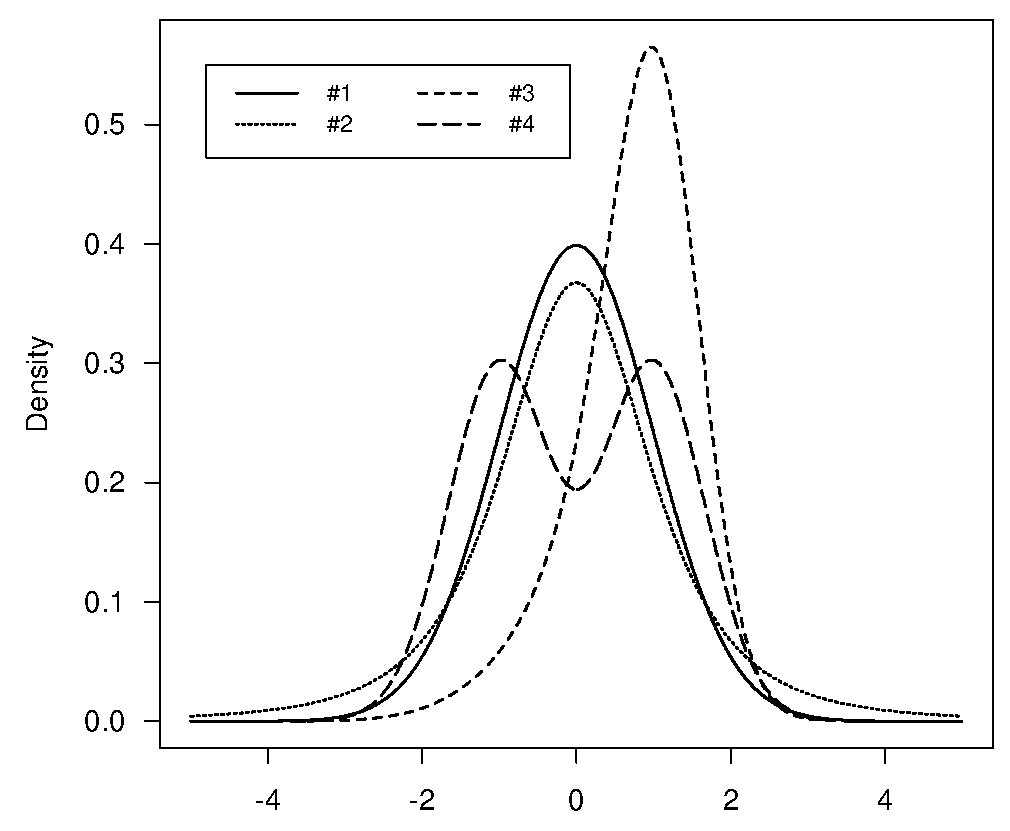
\includegraphics[height=4cm,keepaspectratio=true]{figure_sam.eps}
\caption{Sample figure}
\label{fig:rsxb}
\end{figure}
\end{verbatim}

\begin{figure}[t]
\centering
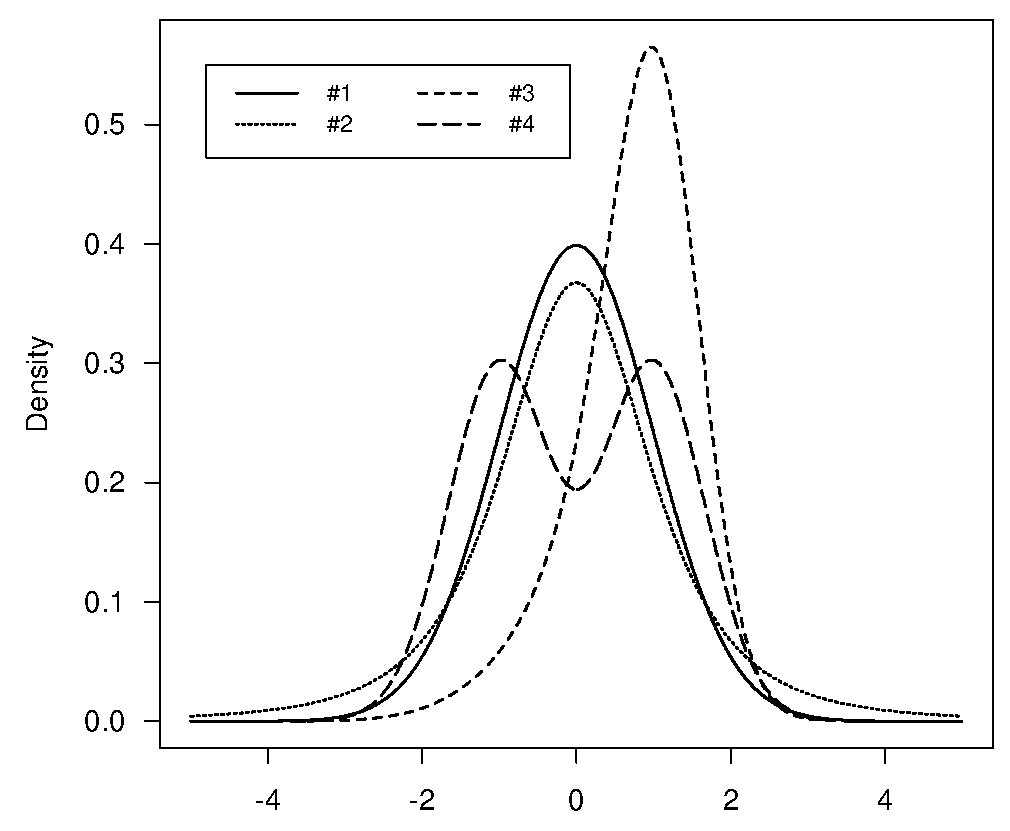
\includegraphics[height=4cm,keepaspectratio=true]{figure_sam.eps}
\caption{Sample figure}
\label{fig:rsxb}
\end{figure}

Similarly you can produce a table using commands something like:
\begin{verbatim}
\begin{table}[t]
\footnotesize
\centering
\caption{Structure of data.}\label{tb:data1}
\tabcolsep=35.5pt
\begin{tabular}{ccccc}
\hline \hline
\multirow{2}*{$N$} & \multicolumn{4}{c}{factor level} \\\cline{2-5}
 & 1 & 2 & $\cdots$ & $I$ \\\hline
1        & $x_{11}$ & $x_{21}$ & $\cdots$ & $x_{I1}$ \\
2        & $x_{12}$ & $x_{22}$ & $\cdots$ & $x_{I2}$ \\
$\vdots$ & $\vdots$ & $\vdots$ & $\ddots$ & $\vdots$ \\
$n$      & $x_{1n}$ & $x_{2n}$ & $\cdots$ & $x_{In}$ \\
\hline \hline
\end{tabular}
\end{table}
\end{verbatim}

\begin{table}[t]
\footnotesize
\centering
\caption{Structure of data.}\label{tb:data1}
\tabcolsep=35.5pt
\begin{tabular}{ccccc}
\hline \hline
\multirow{2}*{$N$} & \multicolumn{4}{c}{factor level} \\\cline{2-5}
 & 1 & 2 & $\cdots$ & $I$ \\\hline
1        & $x_{11}$ & $x_{21}$ & $\cdots$ & $x_{I1}$ \\
2        & $x_{12}$ & $x_{22}$ & $\cdots$ & $x_{I2}$ \\
$\vdots$ & $\vdots$ & $\vdots$ & $\ddots$ & $\vdots$ \\
$n$      & $x_{1n}$ & $x_{2n}$ & $\cdots$ & $x_{In}$ \\
\hline \hline
\end{tabular}
\end{table}

\section{References}

The references cited in your article should be provided within reference environment. An example
of references(book, journal, paper) is given below:
\begin{verbatim}
\begin{reference}
\item[] Box GEP and Draper NR (1969). {\em Evolutionary Operation},
        John Wiley \& Sons, New York.
\item[] Wald A (1949). Note on the consistency of the maximum likelihood
        estimate, {\em Annals of Mathematical Statistics}, {\bf 20}, 595--601.
\item[] Seking JW (2005). Forecasting item production with ARIMA model,
        {\em Technical Paper}, Available from: http://tech.journal.net/2005/
        05102.pdf
\end{reference}
\end{verbatim}

Traditionally the reference should be placed at the end of paper.

{\appendix
\section*{Appendix Title}

There are three types of display methods.

First, there is no title of appendix.
\begin{verbatim}
\appendix
\section*{}
\end{verbatim}

Second, there is a title of appendix.
\begin{verbatim}
\appendix
\section*{Title}
\end{verbatim}

Third, there are more than one title.
\begin{verbatim}
\appendix
\section{Title1}
...
\section{Title2}
\end{verbatim}}

\section*{Acknowledgement}

We are grateful to the ..........

 \begin{reference}
\item[] Box GEP and Draper NR (1969). {\em Evolutionary Operation},
        John Wiley \& Sons, New York.
\item[] Wald A (1949). Note on the consistency of the maximum likelihood
        estimate, {\em Annals of Mathematical Statistics}, {\bf 20}, 595--601.
\item[] Seking JW (2005). Forecasting item production with ARIMA model,
        {\em Technical Paper}, Available from: http://tech.journal.net/2005/
        05102.pdf
\end{reference}

\end{document}
